\capitulo{4}{Técnicas y herramientas}

Dentro de las diferentes herramientas que utilizaré para la realización de este trabajo, la más importante es aquella con la cual realizaré la conversión a JavaScript. Es por ello esencial hacer una buena elección comparando y analizando la diferentes posibilidades a elegir.

Como principales herramientas para la conversión de Java a JavaScript he podido encontrar GWT (Google Web Toolkit), JSweet, WebSwing, Vaadin y DukeScript. Aunque también hay otras, como Rhino\footnote{\url{https://github.com/mozilla/rhino?files=1}}, que descartamos por su poca relevancia o información.

\section{GWT}

\emph{Google Web Toolkit} es un framework ampliamente conocido por los desarrolladores web, entre otras cosas, gracias a ser de código abierto, de su gran utilidad y calidad además de ser completamente gratuito\footnote{\url{http://www.gwtproject.org/}}.
Contiene una SDK que proporciona un conjunto de APIs de Java que permiten el desarrollo de aplicaciones AJAX (\emph{Asynchronous JavaScript And XML}) escritas en Java. Posteriormente compila el código en JavaScript ya optimizado dando rapidez a la aplicación web. 

AJAX es una técnica que se emplea en el desarrollo web, para ejecutar aplicaciones en el lado del cliente en el navegador, comunicándose de manera asíncrona con el servidor. Todas las comunicaciones que se hacen en GWT por medio de RPC son asíncronas, esto quiere decir que las peticiones no se bloquean unas a otras mientras están esperando respuesta, y una vez recibidas, se ejecutan en segundo plano.

Básicamente, permite a los desarrolladores compilar código Java en archivos JavaScript ya optimizados de forma autónoma, proporcionando así todas las ventajas de las aplicaciones escritas en este último lenguaje. 

GWT permite compartir código escrito en Java en la parte del servidor con código JavaScript en la parte del cliente lo que nos lleva pensar que la aplicación resultante será fiel a la idea inicial del Thoth. 

Nos decantamos por GWT porque, a parte de que supone un aprendizaje para mí como alumno, también es la base de otros \emph{frameworks} de los que más tarde hablaré. Ha sido muy utilizado anteriormente y ahora está digamos que en decadencia. El soporte actual es mínimo y sobre todo en el tema visual anda algo anticuado. En el desarrollo del proyecto hemos llegado a ver  y probar <<\emph{bugs}>> que según otros usuarios ya descubrieron hace un par de años.

Aun así, hay bastante información con la que he podido trabajar, y una comunidad grande, que aunque ahora se ha <<pasado>> a otros \emph{frameworks} más actuales, han dejado huella y soluciones a muchos de los problemas con los que he trabajado.

\section{WebSwing}

En cuanto a esta herramienta, es algo diferente a las demás. WebSwing\footnote{\url{http://webswing.org/}} la descubrimos debido a una duda que nos surgió al principio del proyecto. Y es que la aplicación Thoth original cuenta con muchísimos elementos de la biblioteca gráfica <<\emph{Swing}>>, es digamos toda la estructura visual que utiliza. El problema surgió cuando al programar en GWT no podíamos hacer uso de ella, ya que, al ser algo visual debe ir en la parte del cliente y como ya hemos mencionado, es donde se hace la traducción a JavaScript. 

Se trata de un servidor web que permite la ejecución de aplicaciones que utilicen la biblioteca gráfica Swing desde el navegador, utilizando sólo HTML5. De esta forma toda la aplicación de Thoth se ejecutaría en el navegador conservando su aspecto de siempre y manteniendo las ventajas de una aplicación web.

Lamentablemente, esta herramienta se descubrió cuando el proyecto ya estaba muy avanzado. Decidimos entonces continuar por la senda marcada en un principio. Se hizo alguna prueba para ver su funcionamiento y los resultados fueron muy buenos.

Además, utilizar esta herramienta no hubieran supuesto ningún reto como informático y facilitaría tanto el proyecto que este quedaría en nada más que
unas simples mejoras de Thoth hechas con poco desarrollo. Por lo tanto, la descartamos después de haberla probado.

\section{JSweet} 

JSweet\footnote{\url{http://http://www.jsweet.org/}} es básicamente un <<transpiler>>, es decir, un compilador que traduce un código en un lenguaje a otro lenguaje. Al igual que GWT está orientado a objetos, que proporciona una programación segura gracias a que usa un sistema de <<tipado>> Java.

La diferencia fundamental con GWT es que al ser un <<transpiler>> hace una traducción directa entre Java y JavaScript posicionando el código a un lado o al otro del cliente y el servidor. Esto, claramente, tiene sus ventajas y sus inconvenientes dependiendo del uso que se le quiera dar. 

Sin embargo descartamos JSweet por varias razones. En primer lugar porque su traducción de Java a JavaScript es muy literal y no es lo que buscábamos ya que de esa forma perderíamos mucha información.	No reconoce las librerías utilizadas en Thoth. Nos pareció más útil utilizar un cliente servidor en GWT en el cual se pudiera comunicar vía RPC el cálculo del parser. Es decir, con JSweet deberíamos haber reescrito el parser de una forma muchísimo más compleja para que JSweet lo pudiera interpretar y eso hubiera llevado mucho más tiempo. Está mucho mas centrado en el desarrollo en JavaScript en vez de en Java, lo que no nos serviría para poder aprovechar el trabajo de Thoth ya hecho. Recordemos que Thoth esta compuesto por dos versiones, hechas en grupos de dos alumnos y rehacer la aplicación completa en JavaScript sería una tarea muy costosa.

GWT en comparación, cuenta con una comunidad y un soporte bastante más completo, y pensado para desarrolladores Java, con una gran documentación acerca de su uso e implementación.

\section{DukeScript}

Se define como una tecnología para la creación de aplicaciones Java <<multi-plataforma>> que internamente hacen uso de tecnologías HTML5 y JavaScript para el renderizado\footnote{\url{https://dukescript.com/}}.
Al igual que en los casos anteriores <<sólo>> se necesita desarrollar la aplicación en Java para después transformarla. Y digo <<sólo>> porque eso es en la teoría ya que como hemos podido ver, y en parte es lógico, la traducción suele requerir, por lo menos, realizar ajustes del lenguaje para un buen funcionamiento.

DukeScript se centra sobre todo en el desarrollo más que en el paso de Java a JavaScript. Da la posibilidad de que alguien con conocimientos, digámoslo así, en Java pueda llevar a cabo un proyecto en lenguajes pensados para aplicaciones móviles o web. Esto no quita que se puedan realizar aplicaciones de escritorio con JavaScript.

\section{Vaadin}

Vaadin en un \emph{framework} de Java de código abierto, para crear aplicaciones web\footnote{\url{https://vaadin.com/home}}. Se programa en Java o cualquier otro lenguaje de JVM o Java Virtual Machine. Lo más destacado de Vaadin es que está construido sobre una base de GWT, por ello es una de las grandes alternativas a este último. La forma de trabajar con Vaadin es mediante el lenguaje Java e incorpora un lado cliente y otro servidor, en el cual irán las funcionalidades más complejas y su programación es dirigida por eventos. Es decir, hasta aquí es igual a GWT.

Las mejoras con respecto a GWT son varias, pero voy a mencionar solo aquellas que son más relevantes para este proyecto. Cuenta sobre todo con muchos elementos visuales, mejorados y con diseños más actuales. La parte visual es tan importante en Vaadin que incluyen un <<diseñador>>\footnote{\url{https://vaadin.com/designer}} o \emph{designer} en inglés, como complemento de Eclipse que facilita mucho la creación de la parte visual, ya que da la posibilidad de hacer el diseño de forma visual.

En realidad, la mayor parte de los elementos visuales, menús, \emph{boards}, diagramas estadísticos, iconos etc, están pensados sobre todo para un uso comercial orientado sobre todo para empresas. Por ello, el problema principal es que para poder hacer uso de su potencial se necesitan licencias de pago.

Aunque cuenta con un núcleo de elementos gratuitos y periodos de prueba también gratuitos, decidimos seguir nuestro camino, por llamarlo así, con GWT y hacerlo completamente de esta forma.

Las diferencias con GWT radican sobre todo en el lado de ejecución de la mayor parte de la aplicación. Con GWT, la mayor parte de las operaciones se encuentran en el lado del cliente, mientras que en Vaadin, el lado del cliente se comunica casi con cada interacción con el servidor. Como consecuencia, GWT es más rápido y se percibe sobre todo en condiciones en las que la conexión es mala o está sobrecargada. Por otro lado, Vaadin al ejecutarse sobre todo en el servidor, las operaciones son más seguras, ya que se encuentran más ocultas de cara al usuario. Además, al ser las operaciones en el servidor puede usar cualquier librería estándar de Java, GWT sin embargo, al estar casi todo en el cliente, debe limitarse a unas pocas librerías\footnote{Véase \url{http://www.gwtproject.org/doc/latest/DevGuideCodingBasicsCompatibility.html}}.

Para aclarar un poco las diferencias que hay entre Vaadin y GWT utilizaré una tabla comparativa \ref{tab:comparativa}.



\begin{table}[]
\centering
\begin{tabular}{@{}
>{\columncolor[HTML]{FFFFFF}}p {.33\textwidth} p {.33\textwidth}  p {.33\textwidth}@{}}
\toprule
 
\textbf{Características}   & \textbf{Vaadin} & \textbf{GWT} \\ \midrule
\midrule

\textbf{Lenguaje}         & Cualquier JVM & Java con limitaciones de librerías en la parte del cliente.
 \\ \midrule
\textbf{Ejecución}   & Cliente o Servidor indistintamente  & Se debe diferencias que partes del código van en el cliente y cuales en el  servidor. Esto depende de lo que admita el cliente.
 \\ \midrule
\textbf{Componentes gráficos}     & Librería UI con componentes modernos y mucha variedad & Librería algo anticuada y con fallos.\\ \midrule
\textbf{Herramientas de diseño GUI}  &  Incluye \emph{Designer}  & Manual. Existen herramientas externas de uso comercial con coste.\\
\midrule
\textbf{Tipo de licencia}  & Comercial para la mayoría de los componentes & Gratuita\\ 
 \\ \bottomrule
\end{tabular}
\caption{Tabla comparativa entre Vaadin y GWT.}
\label{tab:comparativa}
\end{table}





\section{Herramientas para el cifrado de contraseñas}

En este programa utilizamos una técnica muy simple, que mejora un poco este aspecto. Sabemos que existen técnicas más avanzadas que lo que aumentan mucho los tiempos de procesado en los ataques por fuerza bruta, por ejemplo. Pero no queríamos centrarnos mucho en ese tema además de que percibimos un ralentizado a la hora de registrar a un usuario ya que cifrar la contraseña requiere un mayor tiempo de ejecución.

La técnica que empleamos se conoce como el cifrado hash con sal o semilla (según su traducción del inglés, \emph{hashing with salt}). Consiste en añadir un conjunto de caracteres aleatorio y concatenarlo a la contraseña y una vez hecho esto, cifrarlo con la función \emph{hash}. De esta manera se consigue que la contraseña sea mucho más aleatoria que la que inicialmente ha introducido el usuario. Además de forma transparente para él. 

Para generar el \emph{salt} en Java contamos con el paquete <<security>> y la clase <<SecureRandom>>\footnote{\url{https://docs.oracle.com/javase/7/docs/api/java/security/SecureRandom.html}} con la que nos aseguramos de crear una cadena de bytes aleatoria. Suficientemente aleatoria para nuestro propósito. Podemos especificar el tamaño en bytes del salt. Para almacenarlo, lo pasamos a formato <<String>>. 


Por otro lado, para hacer la autentificación del usuario se debe almacenar en la base de datos tanto el \emph{salt} como el \emph{hash} generado. Cuando el usuario introduce la contraseña para iniciar sesión, internamente se añade el salt a la contraseña introducida, se cifra con el mismo método y se comparan. Si coinciden, accederá a la aplicación, sino, deberá introducir de nuevo los datos necesarios.



\section{Plataforma \emph{Google Cloud}}


La aplicación cuenta con una base de datos en la que se guarda el registro de los usuarios. A la base de datos se puede acceder desde la plataforma \emph{Google Cloud} con una cuenta creada para ese propósito.

Esta plataforma sirve para alojar aplicaciones realizadas con alguna de las  herramientas de desarrollo web de Google. Se ofrecen varios servicios interesantes, como una base de datos SQL, necesaria para hacer el registro e inicio de sesión.

De esta forma, gracias a la SDK de App Engine podemos gestionar una pequeña base de datos con el \emph{datastore} de Google. Se trabaja con entidades y para este proyecto se han creado 3 tipos de entidades.

\begin{itemize}
\item \textbf{User}. En ella se almacenan los usuarios registrados con un nombre, \emph{email}, fecha de registro y contraseña (\emph{password}). Además, como ya hemos hablado en la sección Herramientas para el cifrado de contraseñas, también una \emph{salt} para hacer el inicio de sesión (ver figura \ref{fig:4.1}).
\item \textbf{UserAction}. Se muestra la fecha de la última sesión de cada usuario. Con esta entidad pretendemos ver que usuarios son más activos, cuando se ha utilizado etc. Es cierto que esto se puede analizar desde el administrador de \emph{Google Cloud}, pero decidimos introducir esta entidad antes de alojarla ahí.
\item \textbf{GrammarUsed}. Entidad que sirve para almacenar las gramáticas comprobadas por un usuario. 
\end{itemize}

\begin{figure}[h]
\centering
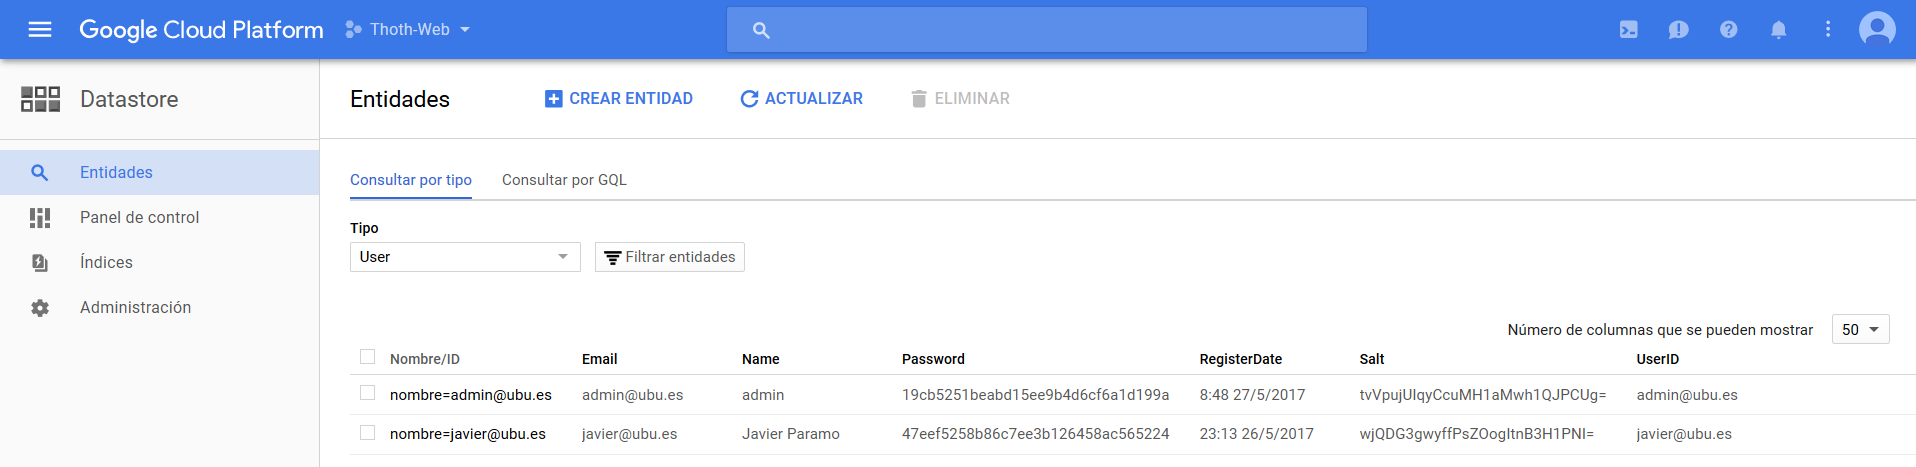
\includegraphics[width=0.99\textwidth]{BaseDatos-user}
\caption{Base de datos en \emph{Google Cloud}. Se puede apreciar la entidad <<User>> que muestra la base de datos.}
\label{fig:4.1}
\end{figure}

La aplicación se puede gestionar fácilmente desde esta plataforma, el problema principal es que es de pago, pero cuenta con una versión gratuita de un año completo, con un gasto máximo de 300 euros. Esto quiere decir que puedo utilizar elementos con coste adicional hasta llegar al cupo de los 300 euros. 
